%%% fs-seim-stream - Stream processing concepts

\label {fs-stream}

In this section we formalize stream processing model. It allows us to use unified terms and to avoid binding to the specific implementation. At the same time, proposed model is realistic enough to be applicable  for industrial solutions.

Commonly, stream processing system is shared-nothing distributed runtime that handles potentially unbounded number of input events and process them one-by-one according to the procedures provided by user. The main purpose of this kind of data processing systems is to provide low latency between event occurrence and its processing. Term {\it distributed} %means
implies 
 that processing can be scaled horizontally, i.e. user's procedures can have partitions on distinct computational units or shards. The following subsections detail the properties of such system more precisely.  

\subsection{Data flow}
The main data flow abstraction is a {\it stream}. Stream is an infinite sequence of events or data items. Each data item consists of payload defined by user and meta-data. For simplification, we assume that all items get into the stream through single input called {\it front}. Meta-data is assigned when item arrives to the front. Meta-data is usually just a current UNIX timestamp in milliseconds. The output data items (if any) leave stream through single {\it barrier}. High-level view of the stream concept is shown in the figure ~\ref{data-flow}.

\begin{figure}[htbp]
  \centering
  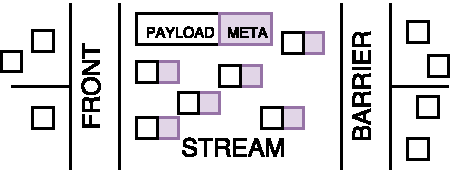
\includegraphics[width=0.48\textwidth]{pics/stream}
  \caption{Data flow}
  \label {data-flow}
\end{figure}

\subsection{Ordering model}
It is assumed  that there is total order on meta-data, and meta-data lables are  assigned to incoming items  monotonically.

\subsection{Computation flow}
Similarly to the most stream processing systems, our model assumes that computational pipeline is defined in the form of {\it execution graph}. The vertices of execution graph are operations, and edges are links between them. 

\subsection{Operations}
We assume that the set of basic operations are complete enough to express {\it reduce} operation in terms of MapReduce framework.

\subsection{Physical deployment}

BN: How {\em strict restrictions} are defined? Have you ANY restrictions?

Generally, we do not have strict restrictions regarding physical execution of the data flow.  
Nevertheless, we assume that each operation can be partitioned between multiple shards. Partitioning can be applied by key extracted from item's payload for stateful operations or randomly for stateless. Regarding physical links between operations, we suppose that they guarantee FIFO order.

\subsection{Guarantees}

BN: If we do not require something, then why it is mentioned? 

We do not require any guarantees on data processing. At the same time, it should be noted that ordering properties can be important for guarantees satisfaction within specific tasks.